%% ****** Start of file aiptemplate.tex ****** %
%%
%%   This file is part of the files in the distribution of AIP substyles for REVTeX4.
%%   Version 4.1 of 9 October 2009.
%%
%
% This is a template for producing documents for use with 
% the REVTEX 4.1 document class and the AIP substyles.
% 
% Copy this file to another name and then work on that file.
% That way, you always have this original template file to use.

%\documentclass[aip,graphicx]{revtex4-1}
%\documentclass[aip,reprint]{revtex4-1}

%\usepackage{graphicx}

%\draft % marks overfull lines with a black rule on the right
%\documentclass[pre,aps,floatfix,authordate1-4,twocolumn]{revtex4-1}
%\documentclass[pre,aps,floatfix,authordate1-4]{revtex4-1}

\documentclass[aps,prl,superscriptaddress,twocolumn]{revtex4}



%\documentclass[aps,prl,preprint,groupedaddress]{revtex4}

\usepackage{rotating} 
\usepackage{times}
\usepackage{graphicx}
\usepackage{setspace}
\usepackage{amsmath}
\usepackage[obeyFinal]{easy-todo}
\begin{document}

% Use the \preprint command to place your local institutional report number 
% on the title page in preprint mode.
% Multiple \preprint commands are allowed.
%\preprint{}

\title{Atomistic resolution structure and dynamics of lipid bilayers in simulations and experiments} %Title of paper

% repeat the \author .. \affiliation  etc. as needed
% \email, \thanks, \homepage, \altaffiliation all apply to the current author.
% Explanatory text should go in the []'s, 
% actual e-mail address or url should go in the {}'s for \email and \homepage.
% Please use the appropriate macro for the type of information

% \affiliation command applies to all authors since the last \affiliation command. 
% The \affiliation command should follow the other information.

\author{O. H. Samuli Ollila}
\email[]{samuli.ollila@aalto.fi}
%\homepage[]{Your web page}
%\thanks{}
%\altaffiliation{}
\affiliation{Aalto University}


% Collaboration name, if desired (requires use of superscriptaddress option in \documentclass). 
% \noaffiliation is required (may also be used with the \author command).
%\collaboration{}
%\noaffiliation

\date{\today}

\begin{abstract}
% insert abstract here
Abstract.
\end{abstract}

%\pacs{}% insert suggested PACS numbers in braces on next line

\maketitle %\maketitle must follow title, authors, abstract and \pacs

% Body of paper goes here. Use proper sectioning commands. 
% References should be done using the \cite, \ref, and \label commands


%\label{}
\section{Introduction}
\todo{Samuli: Add citations to the introduction}
Atomistic resolution molecular dynamics simulations of lipid bilayers are nowdays
widely used technique to seek answer to various research questions.
Typically interactions between other biological molecules (e.g. proteins, drugs, ions etc.)
and lipids are studied but sometimes also lipid properties are directly under interest.
The questions are often biologically motivated and the atomistic resolutions simulations
gives very detailed information which is experimentally unattainable.

When simulations are used in this kind of studies, it is necessary to understand
the limitations of the method and also the accuracy of the used model.
In the pioneering atomistic resolution lipid bilayer simulations the quality of
the simulation respect to reality was measured mainly by comparing the 
acyl chain order parameters and area per molecule between experiments and
simulations. Especially some simulation models repruced these amazingly well
which led to the wide usage of these models.

%was convincing enough to large amount of scientists who started
%to use simulations as their main or supplementary technique to study lipid bilayers. 

Despite of the success of the models to reproduce the acyl chain properties and
molecular density more or less correctly, already early days it was pointed out
by comparing simulations to various experiments
that the glycerol backbone and choline headgroup order structure may not have been 
correctly described. However, at the time simulations were very short compared
to currently accessible timescles and it was not clear if the molecules had
time to sample all the states the model would predict. Also the method to 
quantitatively measure atomistic resolution molecular dynamics and compare to
simulations was not available, thus the real sampling timescales were not known.
For these reasons the estimates of the quality of headgroup were inconclusive on
the early days of molecular dynamics simulations of lipid bilayers and
the issue has gained more attention only very recently.

While the C-H bond order parameters for all hydrocarbon segments are yet the
core parameter to quantify the lipid model quality, the area per molecule 
is quite generally replaced with form factor.
The main reason is that the area per molecule is calculated from the scattering
data using a model (set of assumptions). Thus, when this value is compared to
the value from simulations, the simulations are not compared directly to experiments
but to a value which comes from another model (set of assumptions to calculate the
area per molecule). For this reason the area per molecule is nowdays replaced
by comparison between form factor from simulations and x-ray or neutron scattering.

In this review we discuss the current state of the art methods to compare the 
atomistic resolution lipid structure and dynamics in simulations to the experiments. 
The C-H bond order parameters measured with NMR and form factors measured
with x-ray or neutron scattering are discussed for structural comparison,
and spin lattice relaxation rates for the comparison of dynamics.
The main advantages of these parameters are that
the experimental techiques are non-invansive, they are measured from multilamellar phase 
which is practically always present in simulations as well due to periodic boundary conditions
and that the compared quantity (order parameter, spin lattice relaxation and form factor) is achieved from 
the actual experimental data in a robust way. The experimental results from these
experimental techniques are also highly reproducible and the measured timescales
are appropriate for the comparison to simulations. Also several other experimental
parameters and techniques are used to quantify the simulation quality, however,
none of these is as robust as order parameters, spin relaxation rates or form factor. The most
commonly used other techniques are shortly discussed in the end of the review.

\section{C-H bond order parameters as atomistic resolution structural measure}

\todo{This is the first sketch of this section. It is composed from the content in the blog
and from the things which came into my mind. A lot of references should be added, the text should polished,
things should be added and checked and figures should be improved. However, the main strucutre and idea of the section should be visible.}

\noindent {\bf Here will be described:}\\[0.1cm]

\noindent How are the order parameters measured.\\
What is the primary experimental observable. \\
How accurate are the experimental results. \\
How order parameter is calculated from simulations. \\
How accurate are the order parameters from simulations. \\
What can be learned about the structure when comparing order parameters between experiments and simulations \\[0.5 cm]

\subsection{Definition and properties of C-H bond order parameter}\label{OPdefinition}
In lipid bilayer systems the order parameter of a hydrocarbon C--H vector is typically defined as 
\begin{equation}\label{orderP}
S_{{\rm CH}}=\frac{1}{2}\langle 3 \cos^2 \theta-1 \rangle,
\end{equation} 
where the angle brackets denote an ensemble average over the sampled conformations, and $\theta$ is the angle between the C--H bond and the membrane normal.
The numerical values of order parameters vary between $-\frac{1}{2} < S_{{\rm CH}} < +1$
depending on the sampled $\theta$ distribution.
The motivation for this definition is its connection to the dipolar and quadrupolar splitting measured with
$^1$H-$^{13}$C NMR techniques and $^2$H NMR techniques, respectively. The definition has a form of
second order lagrangian which arises from fundamental theory of interactions between spin systems~\cite{abragam}.
This theory gives a connection between structures sampled by lipid molecules and experimental observables
through the C-H (or C-D in $^2$H NMR) bond order parameter. However, the connection between structure
and order parameters is not fully uniques since several angle distribution can give the same order parameter.
On the other hand, the order parameter can be uniquely calculated from the known angle distribution.
Thus, the order parameters can be calculated from the suggested structural model and compared against
the experimental values to check the quality of the model but the structural models cannot be directly
build fromt the order parameters. Molecular dynamics simulations is very popular techique to study the
sampled atomistic resolution stuctures of lipids and other biomolecules and comparison of them 
to NMR order parameters has been very useful in order to validate simulation results, and also to interpret
the experiments.

Order parameters give very detailed information about atomistic resolution structure since the values can be
measured with high quantitative accuracy for each C-H bond present in the lipid molecule. 
In most experiments the absolute value is measured, however, also the sign can measured and is known
for several segments.
Especially it should
be noted that the order parameter might have different value for different C-H bonds in the same carbon and
this difference is also detectable in experiments and simulations. In this review we call the phenomenon of 
unequal order parameters for hydrogens attached to the same carbon {\it forking} as done also in our recent work~\cite{botan15}.
This large amount of accurate local information about the structure makes the order parameters 
the best parameter to evaluate atomistic resolution structure of different models against the experiments;
if discprepancy is found in order parameter related to certain bond it is known that the model has problems
in the orientation of this specific bond. This gives order parameters a significant advance over, e.g. other
accurate NMR obervables like ??. These can be also used to quantify the structural quality, however, in the
case of disagreement the problem points in the model are more difficult to localize.


%In sections~\ref{??} and~\ref{??} we review the most relevant experimental and molecular dynamics simulation aspects related to the usage of
%order parameters in order to interpret the atomistic resolution structure of lipid bilayers. In section~\ref{??} we
%discuss the connection between structure and order parameters.



The absolute values of order parameters can be measured by detecting quadrupolar splitting with $^2$H NMR~\cite{seelig77c} or by detecting dipolar 
splitting with $^1$H-$^{13}$C NMR~\cite{hong95a,gross97,dvinskikh05a,ferreira13}. The measurements are based on
different physical interactions, and also the connections between order parameter and quadrupolar or dipolar splitting
are different. 

\subsection{Order parameters from $^2$H NMR experiments}

In the $^2$H NMR experiments the absolute values of order parameters are connected to the measured quadrupolar 
splitting $\Delta \nu_Q$ ($^2$H NMR) through the equation 
\begin{equation}\label{HNMRop}
|S_{{\rm CD}}|=\frac{4}{3} \frac{h}{e^2qQ} \Delta \nu_{{\rm Q}}, 
\end{equation}
where $e$ is the elementary charge, $Q$ is the deuteron quadrupole moment and $h$ is the Planck's constant. 
The parameter $q$ is related to the largest electric field gradient and in practise its value is not known; 
therefore the static quadrupolar coupling constant $\frac{e^2qQ}{h}$ is defined, and its value measured for 
different compounds in their solid state. In C-D order parameter measurements for lipids, it is typical to 
use the value  measured for different alkenes, $\frac{e^2qQ}{h}$=170 kHz. The relation between order parameters 
and quadrupolar splittings then becomes $S_{{\rm CD}}=0.00784 \times \Delta \nu_{{\rm Q}}$.
This relation is useful as many publications report only the quadrupolar splittings. For a review and more accurate description see the work of Seelig~\cite{seelig77c}.

\subsection{Order parameters from $^{13}$C NMR experiments}

In $^1$H-$^{13}$C NMR experiments the dipolar splitting $\Delta \nu_\mathrm{CH}$  is measured. This is then related to
the effective dipolar coupling $d_\mathrm{CH}$ through a scaling factor depending on the pulse sequence used in the 
experiment~\cite{hong95a,gross97,dvinskikh05a,ferreira13}. The effective dipolar coupling $d_{{\rm CH}}$ is 
connected to the absolute value of order parameter through equation
\begin{equation}\label{CNMRop}
|S_{{\rm CH}}|=\frac{4\pi\langle r_\mathrm{CH}^3 \rangle}{\hbar \mu_0 \gamma_h \gamma_c} d_\mathrm{CH}, 
\end{equation}
where $r_{{\rm CH}}$ is the C-H distance, $\mu_0$ is the vacuum permittivity, and $\gamma_h$ and $\gamma_c$ are 
the gyromagnetic constants for $^1$H and $^{13}$C nuclei. In contrast to Eq.~\ref{HNMRop}, all the parameters in 
Eq.~\ref{CNMRop} are in principle known. However, for the internuclear distance only the average $⟨r_{{\rm CH}}⟩$ 
is known, not the third moment $⟨r^3_{{\rm CH}}⟩$. For this reason values between 20.2-22.7 kHz are used for
$\frac{4\pi\langle r_\mathrm{CH}^3 \rangle}{\hbar \mu_0 \gamma_h \gamma_c}$ depending on the original 
authors~\cite{hong95a,gross97,dvinskikh05a,ferreira13}.

\subsection{Quantitative accuracy of experimental order parameter values}

It must be stressed that $^2$H NMR and $^{13}$C NMR are fully independent experiments since the deuterium quadrupolar splitting $\Delta \nu_Q$
and the dipolar splitting $d_{{\rm CH}}$ are different physical observables. In addition, the prefactors connecting the observables to the order 
parameter (Eqs.~\ref{HNMRop} and~\ref{CNMRop}) are independently measured. Further independent experiments are performed With $^{13}$C NMR 
by measuring the $^1$H-$^{13}$C dipolar couplings using different pulse sequences~\cite{hong95a,gross97,dvinskikh05a,ferreira13} when the connection
between dipolar splitting $d_{{\rm CH}}$ and effective dipolar coupling $d_\mathrm{CH}$ is different.

The order parameters measured with different techniques are compared by several authors, see Table 1 by Gross et al.~\cite{gross97}, 
Table 1 by Dvinskikh et al.~\cite{dvinskikh05a}, Table 1 and Fig. 3 by Ferreira et al.~\cite{ferreira13} and Fig. 2 and related discussion
by Botan et al.~\cite{botan15}. The absolute values of order parameters measured with different techniques by independent reasearch groups are in good agreement. 
By comparing different literature values for the choline headgroup and glycerol backbone Botan et al. suggest that order parameters would be known with the accuracy of $\pm$0.02 for
purified PC lipid bilayer samples. The lower order parameter reported in some studies~\cite{??} were suggested to arise from lower experimental accuracy.
Based on this comparison Botan et al. suggested sweet spots where choline and glycerol backbone order parameters should fall in the simulation models, see Fig.~\ref{HGorderparameters}.
\begin{figure}[]
%  \centering
  \includegraphics[width=8.6cm]{../Fig/comparisonSorted.pdf}
\newline
  \caption{\label{HGorderparameters}
  Order parameteres from simulations and experimental values from literature for glycerol and choline groups collected by Botan et al.~\cite{botan15}.
The experimental values were taken from the following publications:
 DMPC 303~K from \cite{gross97},
 DMPC 314~K from \cite{dvinskikh05a},
 DPPC 322~K from \cite{gally75},
 DPPC 323~K from \cite{akutsu81},
 POPC 296~K from \cite{bechinger91}, and
 POPC 300~K from \cite{ferreira13}.
  The vertical bars shown for some of the computational values are not error bars, but demonstrate that for 
these systems we had at least two data sets (see Table 1 in Botan et al.~\cite{botan15});
the ends of the bars mark the extreme values from the sets, and the dot marks their measurement-time-weighted average. 
The interactive version of this figure is available at  https://plot.ly/$\sim$HubertSantuz/72/lipid-force-field-comparison/.
} 
\end{figure}
For acyl chain such systematic comparison of values from different sources has not been done. It seems that for some segments the 0.02 accuracy would
could not be achieved with similar comparison. However, in general also the acyl chain order parameters from different sources are also in good agreement
as demonstrated, e.g. by Ferreira et al.~\cite{ferreira13}, see Fig.~\ref{CHAINorderparameters}.
\begin{figure}[]
%  \centering
  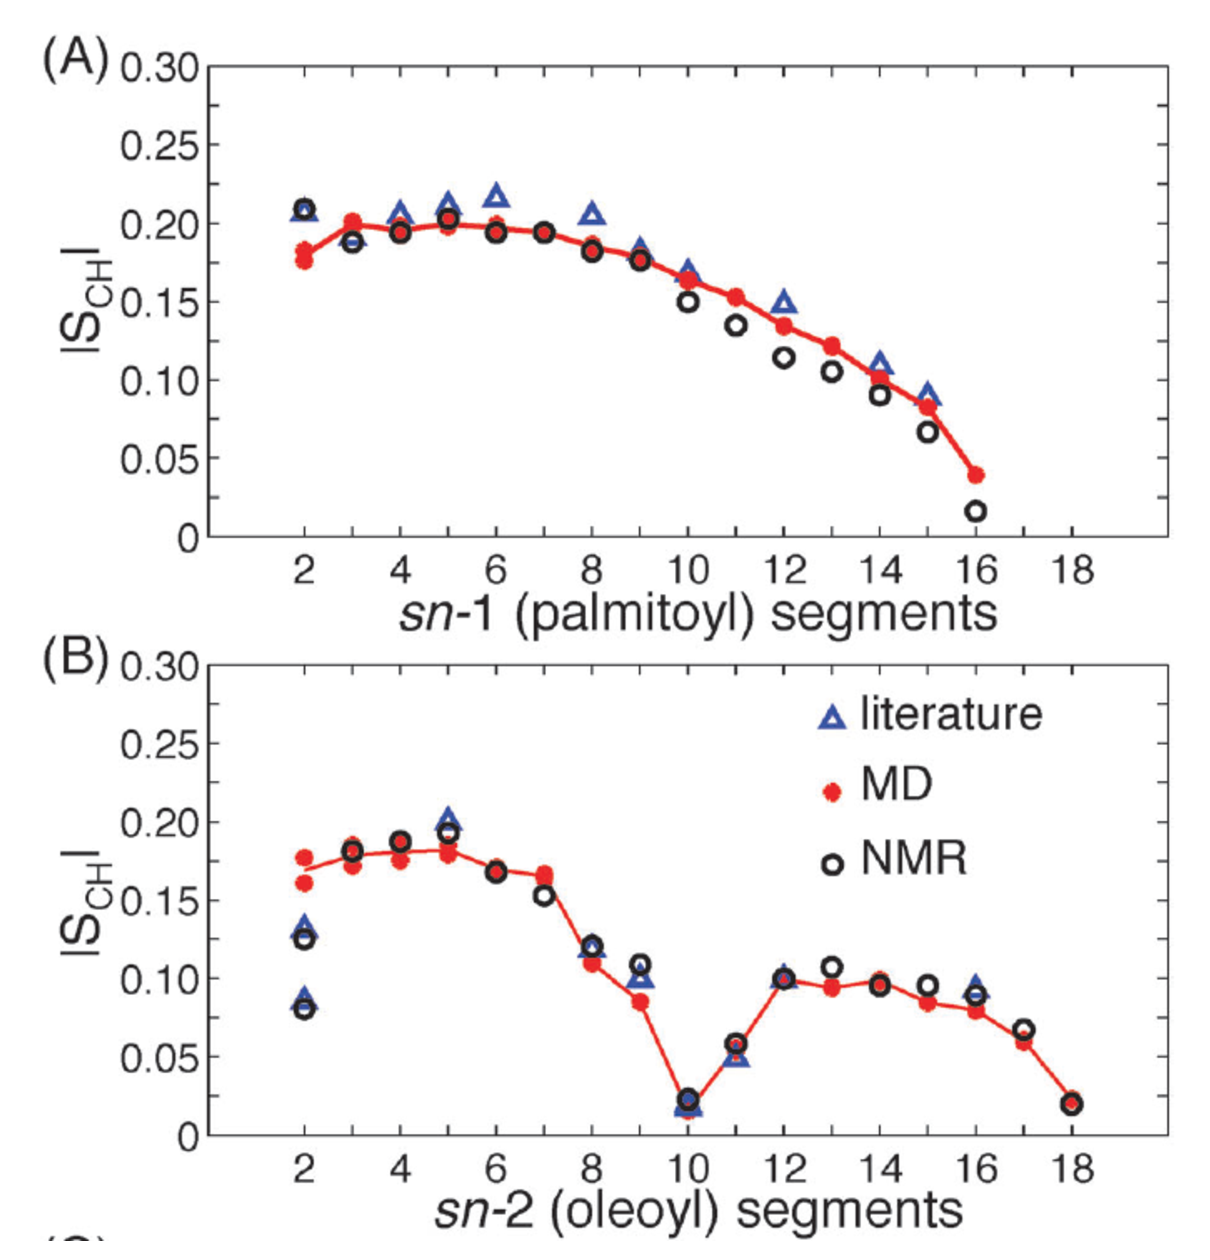
\includegraphics[width=8.6cm]{../Fig/acylCHAINopBYferreira.eps}
\newline
  \caption{\label{CHAINorderparameters}
    Picture adapted from~\cite{ferreira13}.
    Order parameter magnitude $|S_{{\rm CH}}|$ vs. carbon segment number for the
    sn-1 and sn-2 acyl chains of POPC (A and B respectively). Data from fully hydrated POPC at
    300 K obtained with $^1$H–$^{13}$C solid-state NMR (black dots)~\cite{ferreira13} and MD simulations
    (red dots)~\cite{ferreira13}, as well as data from 2H NMR (blue triangles) (sn-1~\cite{seelig78} and
    sn-2~\cite{seelig78,perly85} at 300 K).
} 
\end{figure}

The measurement of quadrupole and dipolar splittings are relatively accurate, especially for quadrupolar splitting.
HOW ACCURATE EXACTLY? Thus the quantitative accuracy of measured order parameters is largely affected by the accuracy 
of the prefactor connecting the measured splittings to the order parameters (Eqs.~\ref{HNMRop} and~\ref{CNMRop}). 
Since the accuracy of these prefactors is single technique is not easy to estimate.
However, comparing the order parameters measured with different techniques based on different physical interactions 
the accuracy of the prefactors can be estimated. Since the order parameters from different techniques are 
almost always within $\pm$0.02 this can be considered to be the quantitative accuracy of the measurements.

\subsection{Qualitative accuracy of experimental order parameter values}

When considering the change of an order parameter with a changing external condition (hydration, ion concentration, etc.), 
the prefactor can be considered to be unchanging. Therefore, the change in a given order parameter, when measured by the 
same people with the same technique and equipment, can be determined in a much higher accuracy than the absolute value of 
the order parameter. We refer to this as the relative accuracy. It is determined by the accuracy of the splitting measurement. 
Especially the very high spectral resolution of the $^2$H-measurements allows the measurement of very small order parameter changes. 
Let us exemplify this with a classical experiment by Akutsu and Seelig~\cite{akutsu81}, where the effect of different ions on 
the quadrupolar splittings of choline headgroup $\alpha$ and $\beta$ segments was measured, see Fig.~\ref{QUADsplitIONeffect}. 
\begin{figure}[]
%  \centering
  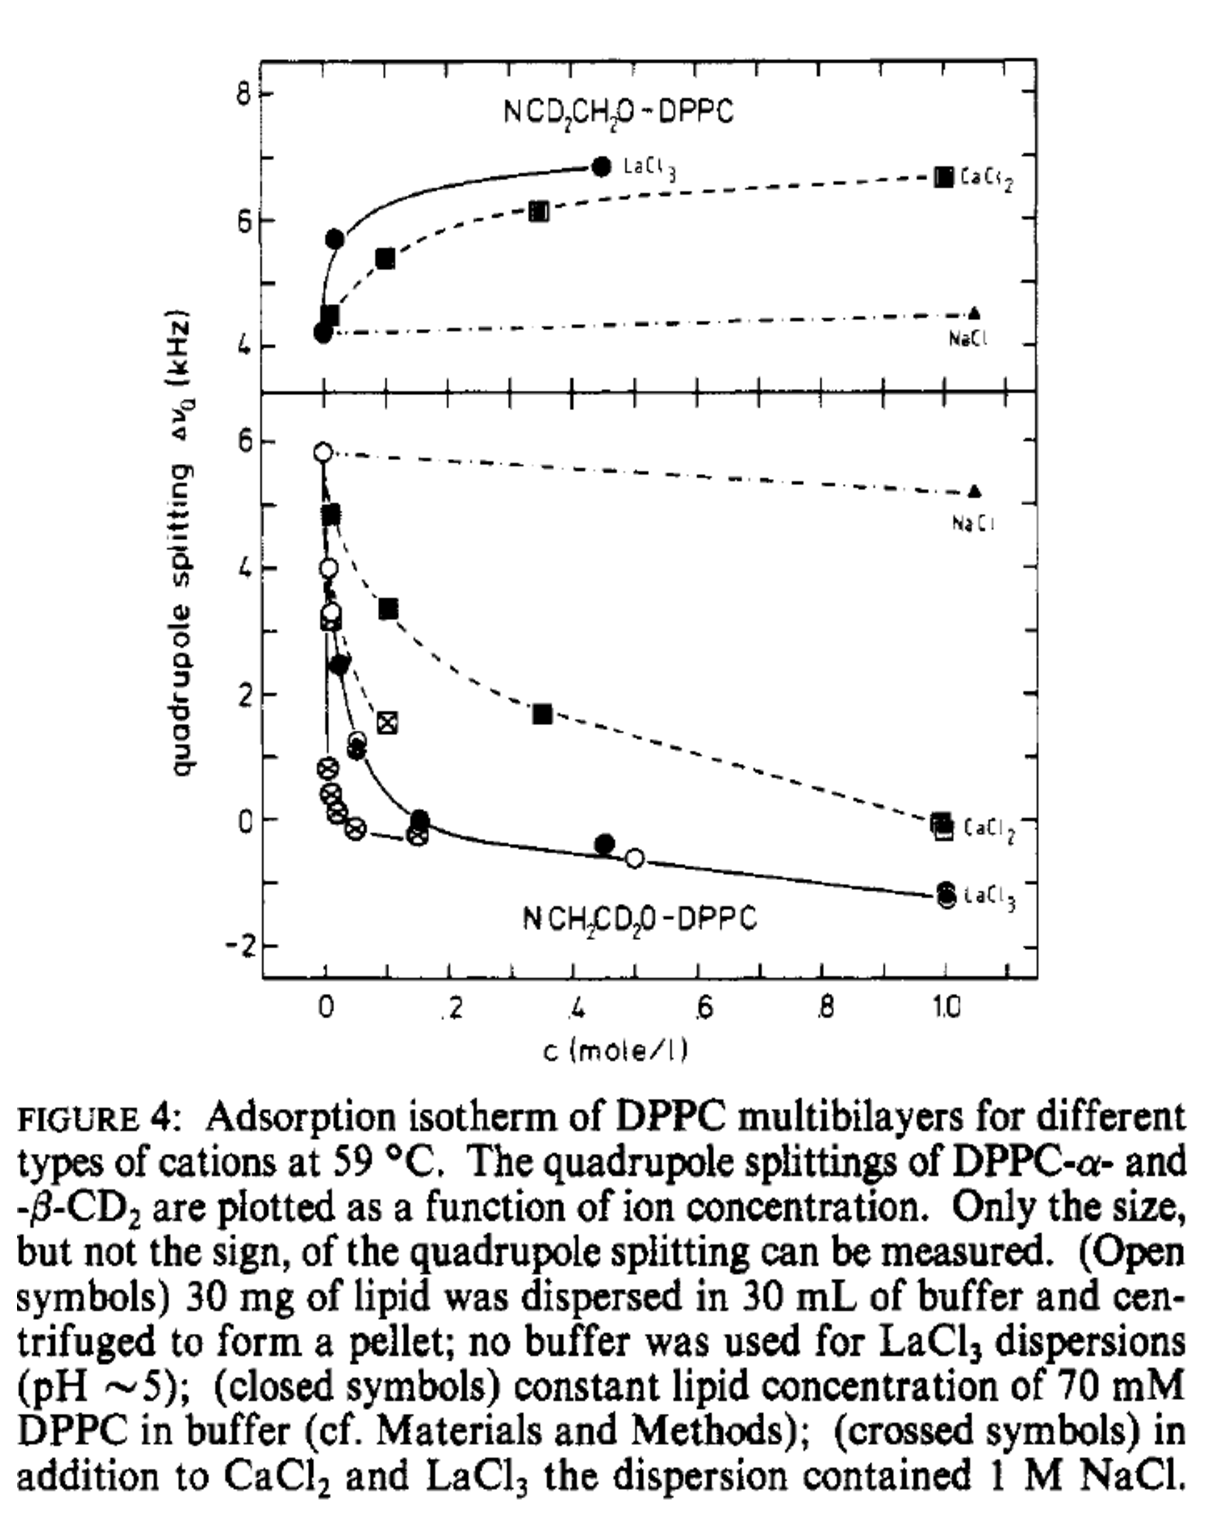
\includegraphics[width=8.6cm]{../Fig/QUADsplitIONeffect.eps}
\newline
  \caption{\label{QUADsplitIONeffect}
    The measured quadrupolar splittings with the explanation in the original caption. 
    Reprinted with permission from Akutsu and Seelig~\cite{akutsu81}. Copyright (1981) American Chemical Society.
} 
\end{figure}

Clearly, the effects of different ions on the quadrupole splittings are differentiable within experimental accuracy in Fig.~\ref{QUADsplitIONeffect}. 
(These changes were later shown to be consistent with the addition of different charges into the bilayer, and the electrometer 
concept was introduced to measure the amount of charge incorporated in the bilayer interface~\cite{scherer89}.) Importantly, 
when the results of Fig.~\ref{QUADsplitIONeffect} are transformed to order parameters in Fig.~\ref{opIONeffect}, 
one can see that the numerical changes in $S_{{\rm CD}}$ are rather small: the y--axis only spans < 0.03 units for $\beta$ and 0.06 for $\alpha$.
\begin{figure}[]
%  \centering
  \includegraphics[width=8.6cm]{../Fig/OrderParameterIONSexp.eps}
\newline
  \caption{\label{opIONeffect}
    Same data as Fig.\ref{QUADsplitIONeffect} but given as order parameters instead of splittings.
  } 
\end{figure}
%Indeed, the measured (upon addition of 1M CaCl2 concentration, the changes due NaCl are negligible) changes in the β-and α-carbons are only ∼ 0.02 and ∼ 0.05, respectively.

The resolution of $^{13}$C NMR experiment depends somewhat on the pulse sequence used. For example Dvinskikh et al. measured the effect of dehydration 
in the lipid order parameters with APM-CP pulse sequence, and changes of 0.01 were measurable~\cite{dvinskikh05b}. Fig.~\ref{opDEHYDeffect} shows the 
order parameters for $\alpha$-and $\beta$-carbons 
as a function of dehydration independently measured with $^{13}$C NMR and $^2$H NMR for different PC lipids. All the results are qualitatively similar, that is, 
they give the same relative change with dehydration.
\begin{figure}[]
%  \centering
  \includegraphics[width=8.6cm]{../Fig/OrderParameterDEHYDexp.eps}
\newline
  \caption{\label{opDEHYDeffect}
    Dehydration changes on $\alpha$ and $\beta$ order parameters measured with different methods. 
    The data taken from Dvinskikh et al.~\cite{dvinskikh05b}, Ulrich et al.~\cite{ulrich94} and Bechinger et al.~\cite{bechinger91}
    Same data as Fig.\ref{QUADsplitIONeffect} but given as order parameters instead of splittings.
  } 
\end{figure}


\subsection{Signs of order parameters}

The absolute values of order parameters are accessible with both $^2$H NMR and $^1$H-$^{13}$C NMR techniques. 
However, only $^1$H-$^{13}$C NMR techniques allow also the measurement of the sign of the order parameter~\cite{hong95a,hong95b,gross97}. 
In older publications that used $^2$H NMR measurements, only the absolute values of the order parameters (or quadrupolar splittings) were discussed 
since the sign was not measurable. For the tail C-H vectors, however, the sign was believed to be negative because $\theta$ was expected to fluctuate 
around 90$^o$ leading to negative order parameters~\cite{seelig77c}. This was later confirmed by using $^{13}$C NMR measurements~\cite{hong95a}. 

The signs of the $^{13}$C-H order parameters have been measured by at least two different techniques and groups: Hong et al. first measured 
eggPC~\cite{hong95a} and then DMPC~\cite{hong95b}; later Gross et al. used a different NMR technique to measure DMPC~\cite{gross97}. 
These experiments are in good agreement with one another and report negative order parameters for almost all the segments, only $\alpha$ and $\gamma$ are positive.
Furthermore, it seems that the signs of choline headgroup and glycerol backbone order parameters~\cite{hong95a,hong95b,gross97} 
and their absolute values~\cite{gally81,ferreira13} are practically unaffected by the acyl tail contents of the bilayers. 
Thus, it can be fairly assumed that the signs of order parameters for all PC lipids in bilayers are the same. 
On the other hand, the positive signs reported for g$_1$, g$_3$ and C$_2$ in acyl chain from $^2$H NMR measurements for DMPC bicelles by Aussenac et al.~\cite{aussenac03}
has generated some confusion in comparison between simulations and experiments~\cite{hogberg08}. However, Aussenac et al. have not actually measured the 
signs but used a model to extract the signs. 

In conclusion, it seems reasonable to assume that the signs measured with $^{13}$C NMR methods~\cite{hong95a,hong95b,gross97}
can be used for all PC lipids in bilayer, i.e. the signs for almost all the carbons are negative, only  $\alpha$ and $\gamma$ are positive.

Typically when the response of order parameters to varying conditions (ions, dehydration and cholesterol) is measured, only the absolute 
values are reported. Where clear responses are observed, like for multivalent ions and dehydration, the experiments are done by gradually 
changing the conditions. The responses of the magnitudes to these changes are systematic, see Figs.~\ref{QUADsplitIONeffect},~\ref{opIONeffect}
and~\ref{opDEHYDeffect}. Thus, it is reasonable to assume that also the signs are not suddenly changing. However, it seems that the sign of 
the $\alpha$ carbon order parameter does change in response to a large amount of bound charge, such as multivalent ions. In this case, 
the absolute value of the order parameter first decreases to zero and then starts to increase again~\cite{altenbach84,seelig87}; 
the behaviour of the spectra has been nicely illustrated by Altenbach et al.~\cite{altenbach84}, see Fig.~\ref{qsCACLeffect}.
\begin{figure}[]
%  \centering
  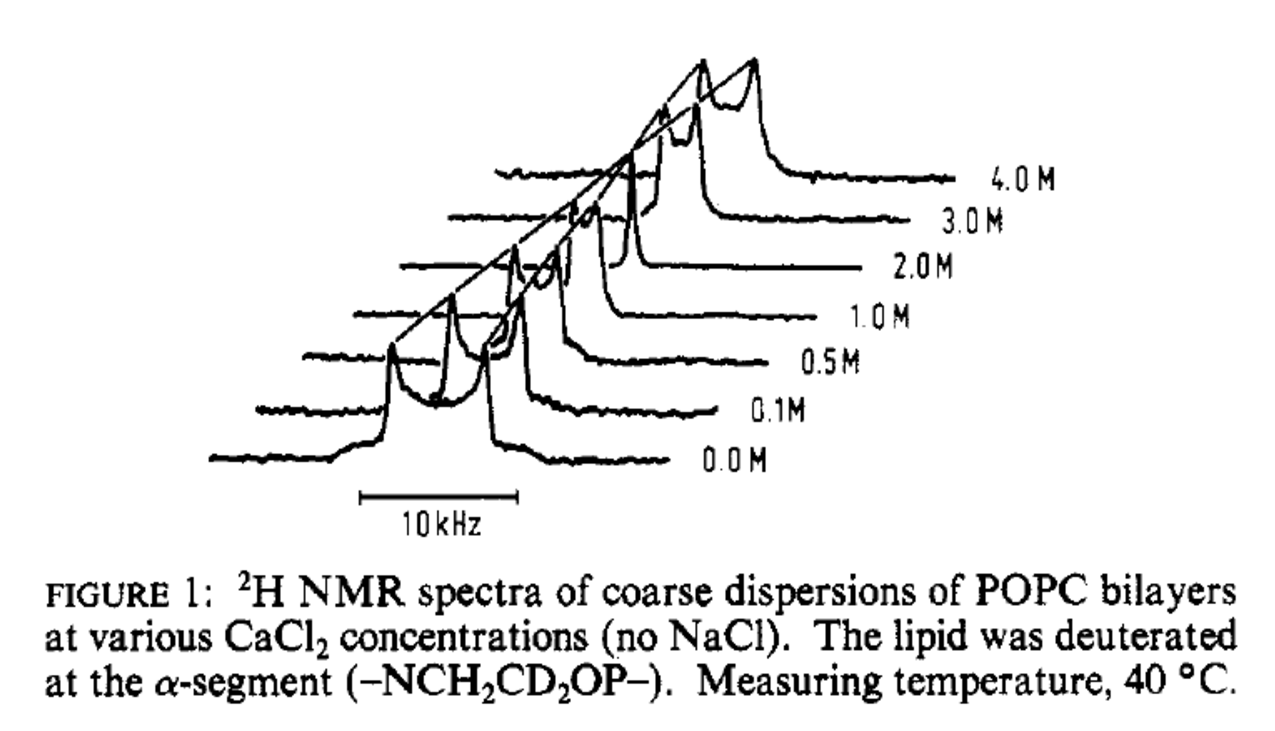
\includegraphics[width=8.6cm]{../Fig/QUADsplitCACLeffect.eps}
\newline
  \caption{\label{qsCACLeffect}
    Quadrupolar splitting $\Delta \nu_Q$ of $\alpha$ of POPC as a function of CaCl$_2$ concentration, related to the order parameter as $S_{{\rm CD}}=0.00784 \times \Delta \nu_Q$. 
    We know nowadays that the order parameter of $\alpha$ in the absense of CaCl$_2$ is positive~\cite{hong95a,hong95b,gross97}.
    Thus, the most obvious interpertation for the result is that the $\alpha$ order parameter decreases to zero when CaCl$_2$ concentration reaches 2.0M, and 
    above these concentrations becomes increasingly negative with further addition of CaCl$_2$. Reprinted with permission from Altenbach and Seelig, Biochemistry, 23, 3913 (1984). Copyright 1984 American Chemical Society.    
  } 
\end{figure}



\subsection{Forking of order parameters}

For most CH$_2$ segments in a fluid phospholipid bilayer, the order parameters of both hydrogens are equal~\cite{seelig74,seelig77,seelig78}.
However, in some cases (e.g., g$_1$, g$_3$, and  C$_2$ carbon in the \textit{sn}-2 chain) the two order parameters are not equal;
this  can be observed with both $^2$H NMR~\cite{seelig75,seelig78,engel81,gally81} and $^1$H-$^{13}$C NMR techniques~\cite{??}. In the present work,
to avoid confusion with the dipolar and quadrupolar splittings in NMR terminology,
we call the phenomenon of unequal order parameters for hydrogens attached to the same carbon {\it forking}. 
Forking has been studied in detail with $^2$H NMR techniques by separately deuterating the R or S position in CH$_2$ segment, and
the studies show that it arises from differently sampled orientations of the two C--H bonds, not from two 
separate populations of lipid conformations~\cite{engel81,gally81}.

\subsection{Order parameter values in the literature}
The acyl chain order parameters are reported extensively in literature for various lipids
in multilamellar phase measured with both $^2H$ NMR and $^{13}$C NMR techniques.
The values are collected in review articles~\cite{leftin11,marsh13}. However, many of the $^2H$ NMR 
studies are measured from lipids with perdeuterated acyl chain(s). In these experiments only numerical
values of order parameters are known but the assignment to the specific carbon is not known.
However, also order parameter measurements from specifically deuterated acyl chain carbon segments 
are done~\cite{seelig74,seelig75,seelig77,seelig78}. In these experiments the assignment is known
but tedious synthesis of specifically deuterated lipids is required.

Also increasing amount of acyl chain order parameters from $^{13}$C NMR are reported in literature~\cite{leftin11,marsh13,ferreira13,??}.
The natural abundance $^{13}$C NMR experiments gives order parameters simultaneously for all the hydrocarbon 
segments. However, in these experiments the assignment of spectral peaks is needed and this is tedious
for acyl chains due to overlap of spectral peaks. This challenge is overcame with careful experiments
and analysis combined to the MD simulations previous specifically deuterated $^2H$ NMR results~\cite{ferreira13,??}.

The agreement between acyl chains order parameters assigned by combining these techiques is very good as shown in Fig.~\ref{CHAINorderparameters}.
Only exception is the simulation results for most models for the C$_2$ segment in sn-2 chain which has forked order parameters
with lower magnitude compared to other segments in the beginnig of acyl chains. This behaviour is systematically observed
to all PC lipid bilayers and it is related to the special conformations of lipid molecules~\cite{??}. 

Also the order parameters for hydrocarbon segments in glycerol backbone and choline are reported in several 
$^2H$ NMR and $^{13}$C NMR studies. The values for PC lipids are recently reviwed in the NMRLipids project~\cite{botan15}.
It should be noted that even the stereospecifity is known for g1 and g3.

There is also increasing amount of order parameter data as a function of changing conditions~\cite{??}.
In the NMRLipids project it was recently demonstrated how this data can be used to check the quality of responses of 
glycerol backbone and choline in MD models, and also the ion partition. This approach has a lot of potential to elucidate 
the quality of different simulation models and also to interpret the experiments. In the NMRLipids project the PC lipid 
dehydration and interactions with ions and cholesterol were compared between different simulation models and experiments. 
Such comparison can be straighforwardly extended to the systems with experimental data available, e.g. other lipids than PC lipids,
to the acyl chain region, to the interactions between, e.g. drugs and poroteins with lipids.

Here we concentrate only directly measured order parameter data from multilamellar samples which correspond typical
MD simulation systems in a box with periodic boundary conditions. The order parameters are reported in the
measured literature also, e.g., for bicelles~\cite{aussenac03,raffard00,sanders92} or from fits to the relaxation
data~\cite{??}. These order parameters can be often related to the ones from multilamellar systems by using
theoretical connections, however, the directly measured order parameters are better for validation of
models due to minimal amount of assumptions used to extract the numerical values.



\subsection{Order parameters from simulations}
In molecular dynamics simulations the trajectories of each atom as a function of time 
are solved by using the Newton's equation of motion and the parameters describing the 
forces between atoms (force field). Also the thermal motion is included in the simulations, thus 
the molecules are expected to sample the realistic phase space during the simulation.
Since the coordinates of all atoms are known from the simuation trajectory,
the order parameters can calculated directly using the definition of Eq.~\ref{orderP}
for each hydrocarbon segment. 

For simulations models without explicit hydrogen atoms 
(united atom models), the hydrogen positions can be generated post-simulationally from 
the positions of the heavy atoms and the known hydrocarbon geometries.
Alternatively, the equations 
??
can be used to calculate the order parameters directly.
These two approaches are almost identical and give essentially the 
same results. However, the Eq.~\ref{??} is valid only for the case where there is no
forking, i.e. order parameters are equal for both hydrogens attached to the 
same carbon.

In general the order parameters for the acyl chain reported from the same
models by different authors are in good agreement in the literature.
The exeption is, however, the order parameters for C-H order parameters
which are calculated incorrectly by the {\it g\_order} program which
is part of the Gromacs package. This discrepancy can be seen
for example by comparing the order parameters between ? (calculated with {\it g\_order}) and ?
(calculated with Eq.~\ref{??} and generating hydrogen positions with {\it protonate}) for
oleyl chain of POPC. In some cases the order parameters are also formally reported 
to be positive~\cite{??}. However, in these cases it almost certain that negative values are
actually achieved from actual calculations. Most likely explanation for reported positive 
values are the missing absolute value lines from the figure label, or the confusion arising
from the fact that the {\it g\_order} gives actually -S$_{{\rm CH}}$.
By takig into account the above mentioned and well understood issues, 
the simulation order parameters for acyl chain in literature are in good
agreement with each others and simulations.

Especially the generally good quantitative agreement between experimental and simulated
order parameters in acyl chain region for pure lipid bilayers (except for C$_2$ segment in sn-2 chain) should be emphasized.
This means that the atomistic resolution structures sampled by the acyl chains are correct
with high probability in the simulations and that the simulations give better and more illustrative
description on acyl chain conformations than the traditionally build models based on NMR data. 
In addition to the quantitatively good agreement in pure bilayers, the changes in 
acyl chain order parameters as a function of changing conditions are generally reasonable.
For example, increase of order parameters as a function of cholesterol concetration and with 
hydration are reproduced in simulations. In contrast the decrease due to addition of
double bonds is also reproduced. It should be noted, however, that the quantitative changes
are often not reproduced correctly when compared. This indicates that even though
the models reproduce atomistic resolution changes into the correct direction, 
the changes are often over or underestimated. There is room for improvement
in the models in this respect. However, in conclusion, the acyl chain 
structure and its qualitative changes are generally well described by the
molecular dynamics simulations and this is one of biggest achievements of the
field, and also one of the most important justification for the usage of such models.

There is more discrepancies in the order parameters and their interpretation reported for glycerol backbone and
choline in the literature. In recent publication from the NMRLipids project~\ref{botan15} the results 
from 12 different models were calculated and compared to the experiments, see Fig.~\ref{HGorderparameters}. 
\begin{figure}[]
%  \centering
  \includegraphics[width=8.6cm]{../../nmrlipids.blogspot.fi/DATAreportediINblog/comparisonSorted.pdf}
\newline
  \caption{\label{HGorderparameters}
    Order parameteres from simulations with different models and experiments for glycerol and choline groups reported by Botan et al.~\cite{botan15}.
    The experimental values were taken from the following publications:
    DMPC 303~K from \cite{gross97},
    DMPC 314~K from \cite{dvinskikh05a},
    DPPC 322~K from \cite{gally75},
    DPPC 323~K from \cite{akutsu81},
    POPC 296~K from \cite{bechinger91}, and
    POPC 300~K from \cite{ferreira13}.
    The vertical bars shown for some of the computational values are not error bars, but demonstrate that for 
    these systems we had at least two data sets (see Ref.~\cite{botan15});
    the ends of the bars mark the extreme values from the sets, and the dot marks their measurement-time-weighted average. 
    An interactive version of this figure is available at  https://plot.ly/$\sim$HubertSantuz/72/lipid-force-field-comparison/.
} 
\end{figure}
In this study significant differences in order parameters and structures were observed between the models,
however, none of the models reproduced the order parameters within experimental error.
This indicates that the simulations models are not in the level that those could be used to
study the glycerol backbone or choline structrure, or phenoma related to their strucuture or
energetics. Despite of the incorrect structures in simulation models the qualitative
responses to the dehydration and charge penetration were qualitatitevly correct. 
However, the ion partition coefficient was significantly off from experiments in
several models. Also the effect of cholesterol on glycerol backbone was overestimated
by the most used model. The conclusions from NMRLipids project and the reported 
numbers differ from some earlier investigations. Some studies have interpreted
essentially same simuation results to be in good agreement with experiments~\cite{??}.
This difference in interpretation seems to arise from the underestimated accuracy
of experimental order parameters. On the other hand, some studies report different
order parameter values than Botan et al. for the same models~\cite{??}.
However, in these studies the order parameter signs and forking are not carefully analyzed
which probably explains the differences. It should be noted that all the data
and analysis by Botan et al. is openly available, so their calculations can 
be carefully re-examinated, which is not the case for other studies.

The statistical error estimates of simulated order parameters are systematically
small. The error of the mean calculated averaging ove time blocks~\cite{ollila07}, independent 
simulations~\cite{poger12} or different lipids~\cite{botain15} all give maximum error $\sim \pm$0.01.

It has been pointed out recently that the sampling of individual dihedral angles might be very
slow compared to the typical (100~ns) simulation timescales~\cite{vogel12}.
After 200~ns, however, even the slowest rotational correlation function of a C--H bond  (g$_1$) reaches
a plateau ($S_\mathrm{CH}^2$) in the Berger model~\cite{berger97}---and, notably,
the dynamics of this segment have been shown to be significantly slower in simulations
than in experiments~\cite{ferreira15}.
In practise,
due to averaging over different lipid molecules,
less than 200~ns of simulation data should be enough for the order parameter calculation;
if the sampling within typical simulation times
is not enough for the convergence of the order parameters,
then the simulation model in question has unphysically slow dynamics.



\subsection{Interplay between simulations through NMR order parameters: Validation and interpretation}

In the above sections we review the accuracy and availability of NMR order parameters in simulations and experiments.
We have concluded that the order parameters for each segments of phospholipids in lipid bilayer are achievable
with high accuracy from simulations and experiments, and also lot of these values are already available 
in the literature. Since the order parameter give very detailed information about the orientations
sampled by C--H bonds in the system.

Why Simulate?
From the experiments it is not clear how large conformational and energetical changes these small changes in the order parameters indicate. This could, however, be revealed with a molecular model that reproduces the measured order parameters. We have already succesfully applied this approach to explain the measured low order parameters (and their temperature dependence) in the lamellar phase of the nonionic surfactant C12E5 [Ferreira et al.]. For the lipid headgroup and glycerol region the problem is, however, that with the current force fields the order parameters from simulation models are both absolutely and relatively too far from the experimental values to be useful for interpretating the experiments. 




Until now, only the absolute values of order parameters have been looked at in the nmrlipids project. However, already the first comment to this blog pointed out the relevance of the signs. (I was a little bit sloppy in my reply and said that the signs of the order parameters are correct in Berger; this is not true as mentioned here and dicussed below). It is important to take the sign into account when the order parameters are discussed in relation to the structure of lipid molecules: Two C-H bonds whose order parameters have the same magnitude but different signs are sampling different orientations. Consequently, the correct signs are crucial if force field parameters are fitted to reproduce the correct order parameters, for example, by using the method suggested by Antti Lamberg in this blog. Thus, I think that from now on we have to start looking also at the signs of the order parameters, not just their magnitude.



\section{C-H bond dynamics from spin relaxation rates and simulations}

\noindent {\bf Here will be described:}\\[0.1cm]

\noindent How the rotational dynamics measured by using NMR relaxation experiments. \\
How the relaxation experiments are connected and compared with simulations. \\
What can be learned and what has been learned about the rotational dynamics from the comparison between spin relaxation and simulations \\[0.5 cm]

\todo{This is quite straightforward to write for me and there is quite good support from our recent work~\cite{ferreira15}.
I will write the first version as soon as I can.}

\section{Stucture factors from scattering and simulations}

\noindent {\bf For this section I would be more than happy for some help} \\[0.1cm]

\noindent {\bf Here will be described:}\\[0.1cm]

\noindent How are the form factors are measured.\\
What is the primary experimental observable. \\

\noindent {\bf On these questions I do not know the answer and it is not exactly clear from where I can find the answers. More specifically:}  \\

\todo{Which is the experimental quantity that the scattering machinary exatcly puts out? \\
How the form factor is determined from the experimental observables? \\
Which assumptions are needed here? \\
There is already some discussion about this in the blog by Peter Heftberger and Georg Pabst, but any kind of information from full 
exaplanation with citations to the hints of relevant literature are helpful here.
The more detailed discussion can be found at:
{\tt https://github.com/NMRLipids/NMRLipids\_V-Review/issues/1}}

\vspace*{5mm}

\noindent How accurate are the experimental form factors. \\

\todo{Has this been discussed in the literature already?
Any kind of information from full exaplanation with citations to the hints of relevant literature are helpful here.
The more detailed discussion can be found at:
{\tt https://github.com/NMRLipids/NMRLipids\_V-Review/issues/2}}

\vspace*{5mm}

\noindent How the form factor is calculated from simulations and compared to experimental ones. \\

\todo{As far as I have understood, the form factor is simply a Fourier transform of electron density. I have some quick and dirty scripts to calculate those in the NMRLipids III repository: \\
{\tt https://github.com/NMRLipids/NmrLipidsCholXray/blob/master/scratch/FFactor/FFstructCALC.sh}\\
{\tt https://github.com/NMRLipids/NmrLipidsCholXray/tree/master/scratch/FFactor}\\
However, I have not been able to install the SIMtoEXP program ({\tt http://link.springer.com/article/10.1007\%2Fs00232-010-9254-5}) so I have not been able to check my script against the standard method.
This should be straighforward issue and should become clear once I check the details. Anyway, any kind of information from full exaplanation with citations to the hints of relevant literature are helpful here.
The more detailed discussion can be found at:
{\tt https://github.com/NMRLipids/NMRLipids\_V-Review/issues/3}}

\vspace*{5mm}

\noindent How accurate are the calculated form factors from simulations. \\

\todo{I think that from statistical point of view accuracy is quite high, however I am not sure about the effect of undulations etc.
Any kind of information from full exaplanation with citations to the hints of relevant literature are helpful here. 
The more detailed discussion can be found at:
{\tt https://github.com/NMRLipids/NMRLipids\_V-Review/issues/4}}

\vspace*{5mm}

\noindent What can be learned about the structure when comparing the form factors between experiments and simulations \\

\todo{I have thought that if the form factor is reproduced by the simulation, the electron density profile should be 
reasonable. However, since some people are tuning the peak highs for better agreement, I am not sure. 
There is also some connection to the thickness. There is already some discussion about this in the blog with
Peter Heftberger and Georg Pabst.
Any kind of information from full exaplanation with citations to the hints of relevant literature are helpful here.
The more detailed discussion can be found at:
{\tt https://github.com/NMRLipids/NMRLipids\_V-Review/issues/5}}



\section{Conclusions}

% Tables may be be put in the text as floats.
% Here is an example of the general form of a table:
% Fill in the caption in the braces of the \caption{} command. Put the label
% that you will use with \ref{} command in the braces of the \label{} command.
% Insert the column specifiers (l, r, c, d, etc.) in the empty braces of the
% \begin{tabular}{} command.
%
% \begin{table}
% \caption{\label{} }
% \begin{tabular}{}
% \end{tabular}
% \end{table}

% If you have acknowledgments, this puts in the proper section head.
\begin{acknowledgments}
% Put your acknowledgments here.
\end{acknowledgments}

% Create the reference section using BibTe
\bibliography{refs.bib}

%\newpage
%\section{APPENDIX: The NMR results reported by Tiago Ferreira}

\listoftodos

\end{document}
%
% ****** End of file aiptemplate.tex ******
